\section{Main matter}

\subsection{Requirements}

\lipsum[1]

\req{req:nolights}{Switch off the lights.}

\lipsum[2]

\req{req:generic_req}{Another requirement.}

\subsection{Questions}

\lipsum[3]

\question{q:where}{Where is the coffee machine?}

\lipsum[4]

\question{q:when}{When is the coffee break scheduled?}


\subsection{References}

\lipsum[5]

\begin{itemize}
\item Sect.~\ref{sec:intro}, Sect.~\ref{sec:scope};
\item \citedoc{AD:ESO-379353}, \citedoc{RD:ESO-363358};
\item \citereq{req:nolights}, \citereq{req:generic_req};
\item \citequestion{q:where}, \citequestion{q:when};
\item Tab.~\ref{tab:test}, Fig.~\ref{fig:m31}, Eq.~\ref{eq:eq};
\end{itemize}


\subsection{Figures and tables}

\lipsum[6]

\begin{figure}[hbtp!]
  \centering
  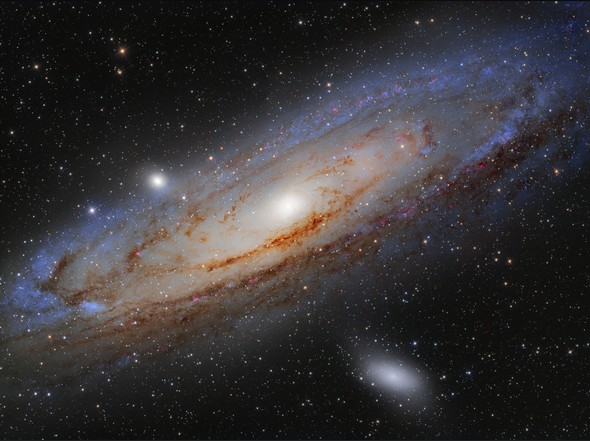
\includegraphics[width=0.5\textwidth]{media/m31}
  \caption{Andromeda galaxy}
    \label{fig:m31}
\end{figure}


\lipsum[7]

\begin{table}[hbtp!]
  \centering
  \begin{tabularx}{\textwidth}{|X|X|X|}
    \hline
    \rowcolor{lightgray} \multicolumn{3}{|c|}{Country List} \\
    \hline
    Country Name or Area Name& ISO ALPHA 2 Code &ISO ALPHA 3 \\
    \hline
    Afghanistan & AF &AFG \\
    \rowcolor{gray}
    Aland Islands & AX & ALA \\
    Albania   &AL & ALB \\
    Algeria  &DZ & DZA \\
    American Samoa & AS & ASM \\
    Andorra & AD & \cellcolor[HTML]{AA0044} AND    \\
    Angola & AO & AGO \\
    \hline
  \end{tabularx}
  \caption{Table to test captions and labels.}
  \label{tab:test}
\end{table}
